بازی زیر را در نظر بگیرید که
$x > 1$،
$x \ne 2$.
\begin{center}
    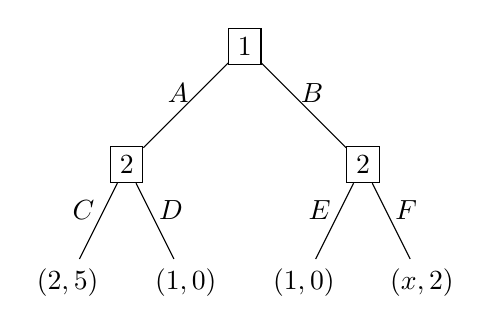
\begin{tikzpicture}
        [level distance=1.5cm,
        level 1/.style={sibling distance=3cm},
        level 2/.style={sibling distance=1.5cm},
        level 3/.style={sibling distance=1cm},]

        \node[rectangle, draw] {$1$}
            child { node[rectangle, draw] {$2$}
                child { node {$(2,5)$} 
                    edge from parent node[left, pos=0.35] {$C$} 
                } 
                child { node {$(1,0)$} 
                    edge from parent node[right, pos=0.35] {$D$}
                }
                edge from parent node[left, pos=0.35] {$A$}
            }
            child { node[rectangle, draw] {$2$} 
                child { node {$(1,0)$} 
                    edge from parent node[left, pos=0.35] {$E$} 
                } 
                child { node {$(x,2)$} 
                    edge from parent node[right, pos=0.35] {$F$}
                } 
                edge from parent node[right, pos=0.35] {$B$}
            } ;

    \end{tikzpicture}
\end{center}

\textbf{الف)}
به ازای مقادیر ممکن برای
$x$،
با استفاده از استفرای بازگشتی،‌ استراتژی‌های تعادل را بیابید.
\vspace{5pt}

\textbf{ب)}
فرم نرمال بازی را بکشید و برای 
$x = 3$
تعادل نش با استراتژی ترکیبی را بدست آورید.